\documentclass[lualatex,paper=a4paper]{jlreq}

% --- パッケージの読み込み ---
\usepackage{luatexja} % 日本語対応
\usepackage{hyperref} % リンク用
\usepackage{graphicx} % 画像用
\usepackage{listings} % コードブロック用
\usepackage{xcolor}   % コード色付け用

% --- ハイパーリンクの設定 ---
\hypersetup{
    colorlinks=true,
    linkcolor=blue,
    urlcolor=blue,
    pdftitle={DevContainerでLaTeXの環境構築}
}

% --- コードブロック（listings）の設定 ---
\lstset{
    basicstyle=\ttfamily\small,
    frame=single,
    breaklines=true,
    columns=fullflexible,
    backgroundcolor=\color{gray!10},
    keywordstyle=\color{blue},
    commentstyle=\color{gray},
    captionpos=b
}

% --- 図表の設定 ---
% 画像の検索パスを設定（必要に応じて）
% \graphicspath{{./images/}}

% --- 文書情報 ---
\title{DevContainerで \LaTeX{} の環境構築}
\author{倶利伽羅らら}
\date{\today}

\begin{document}

\maketitle

また環境構築記事になっちゃいました。「自分用 \LaTeX{} 環境」を作ってみたという話です。あんまり \LaTeX{} には詳しくない（大学のレポートを書くときにトラブったらAI頼り）なので、DevContainerの練習になりました。

\section{DevContainerを用いるメリット}

\subsection{環境構築が高速}
\TeX Liveをインストールするには結構時間がかかります。確か10GB近いファイルをミラーサーバーからダウンロードしています。しかし、Dockerの \href{https://hub.docker.com/r/texlive/texlive}{texlive/texliveイメージ} は2.4GB程度で、DockerHubからのダウンロードで高速です。

\subsection{ホストの環境を汚さない}
Windows版の \TeX Liveを使う場合は、ホームディレクトリに \texttt{.latexmkrc} を置いて、、、ってやるので、設定ファイル等がカオスになりがちです。
また、いつもはLua\LaTeX{} でコンパイルしてるけど、なんかの事情で今日はp\LaTeX{}！って時も、独立した環境を用意できます。

\section{使い方}

\subsection{WSLへのDockerのインストール}
\textbf{※以下のコマンドはWSLで入力してください。}

macOSやLinuxがホストの場合のDockerのインストールが良く分からない、、、のでWindows向けのやり方を紹介します。Ubuntu以外のディストリビューションも良く分からん、、のでUbuntuの場合を紹介します。

Dockerエンジンのインストールは \href{https://docs.docker.com/engine/install/ubuntu/}{公式ドキュメント} を参考にします。

\begin{lstlisting}[language=sh, caption=Dockerのインストールスクリプト]
# Add Docker's official GPG key:
sudo apt update
sudo apt install ca-certificates curl
sudo install -m 0755 -d /etc/apt/keyrings
sudo curl -fsSL https://download.docker.com/linux/ubuntu/gpg -o /etc/apt/keyrings/docker.asc
sudo chmod a+r /etc/apt/keyrings/docker.asc

# Add the repository to Apt sources:
sudo tee /etc/apt/sources.list.d/docker.sources <<EOF
Types: deb
URIs: https://download.docker.com/linux/ubuntu
Suites: $(. /etc/os-release && echo "${UBUNTU_CODENAME:-$VERSION_CODENAME}")
Components: stable
Signed-By: /etc/apt/keyrings/docker.asc
EOF

# Install
sudo apt update
sudo apt install -y docker-ce docker-ce-cli containerd.io docker-buildx-plugin docker-compose-plugin
\end{lstlisting}

\subsection{リポジトリのクローン}
\begin{lstlisting}[language=sh]
git clone git@github.com:sakusan7200/my_docker_latex_env.git
\end{lstlisting}
等でローカル(WSL内を推奨)にクローンします。

\subsection{VSCodeで開く}
さっきリポジトリをクローンした位置まで \texttt{cd} コマンドで移動し \texttt{code .} とします。(VSCodeでWSL内のディレクトリを開いています)

左下の \textbf{＞＜} $\rightarrow$ \textbf{コンテナーで再度開く} を選択し、コンテナに入ります。

% --- 画像の挿入 ---
\begin{figure}[htbp]
    \centering
    % width=0.8\textwidth は行幅の80%に縮小する指定です
    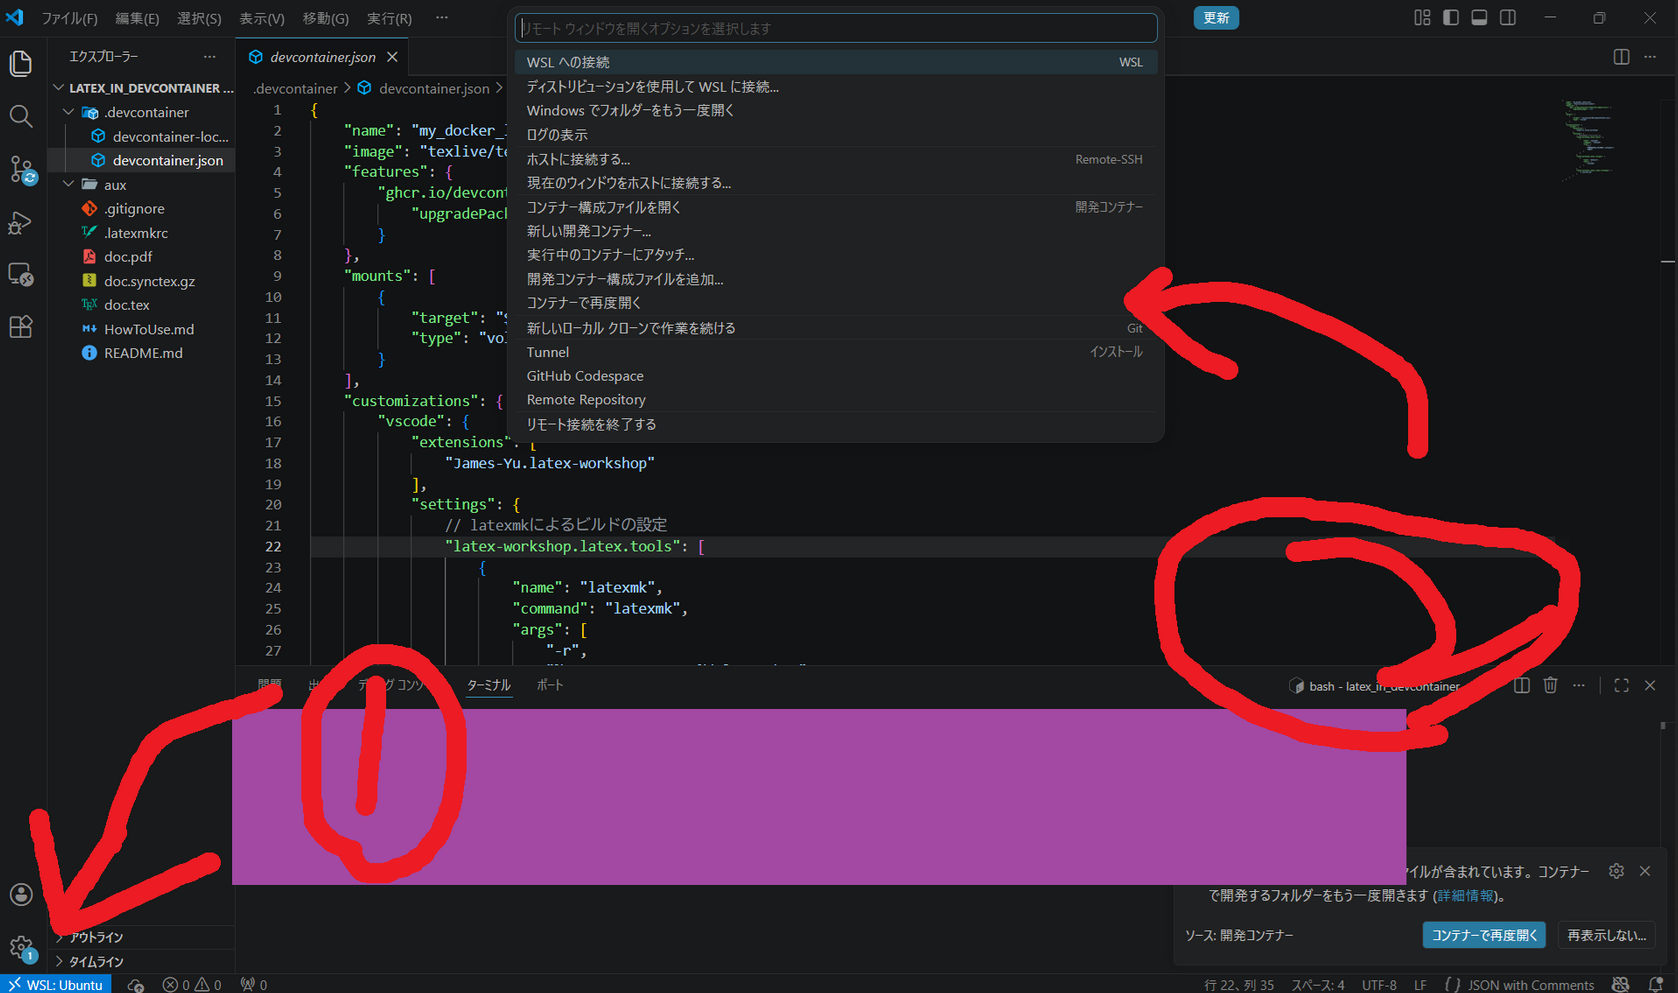
\includegraphics[width=0.8\textwidth]{howto_vscode.png}
    \caption{VSCodeでコンテナを開く操作}
    \label{fig:vscode_reopen}
\end{figure}
% ------------------

\section{アイデア}
以下、自分が何を考えて構築していったのか・気づいたこと書き連ねておきます。

\subsection{ディレクトリ構成}
\begin{lstlisting}
.
├── .devcontainer
│   └── devcontainer.json
├── .gitignore
├── .latexmkrc
└── doc.tex
\end{lstlisting}

\subsection{devcontainer.json}

\subsubsection{features}
\texttt{common-utils} というのを入れてみました。gitとかcurlとか(いい感じに書かれた)\texttt{.bashrc}を入れてくれます。だから、Dockerfileに \texttt{RUN apt install} とかいちいち書かなくて済みます。

\subsubsection{settings}
コンテナを使わないやり方だと、ここの内容をあらゆる文書で共有しカオスになります。ワークスペース直下に \texttt{.latexmkrc} ファイルを作りそこに設定を書いてます。

\subsubsection{Volumeトリック}
\texttt{aux} フォルダには参照の番号付けのための補助ファイルなどが出力されます。バインドマウントによりホストに同期されると多少とはいえリソースを消費するので、除外します。

% エラー回避のため、language=json を language=C に変更
\begin{lstlisting}[language=C, caption=devcontainer.json での volume 設定]
"mounts": [
    {
        "target": "${containerWorkspaceFolder}/aux",
        "type": "volume"
    }
]
\end{lstlisting}

\subsection{.latexmkrc}
上記のVolumeトリックを使うために \texttt{aux\_dir=aux} で \texttt{aux} ディレクトリに諸々を出すようにしてます。

\texttt{-synctex=1} でsynctexを有効にしてます。PDF上で \texttt{Ctrl+ダブルクリック} でtexファイル上の該当箇所に飛べます。逆に、texファイル上で \texttt{Ctrl+Alt+J} でPDFの該当箇所に飛べます。そんな機能あるんですね。知らなかった、無知って怖い。

\texttt{pdf\_mode=4} はlualatexにより直接PDFを作成する指定です。lualatexの場合はdvipdfを通らずにPDFを出力できます。知らなかった、無知って怖い2。

\section{まとめ}
TikZや独自テンプレート、追加パッケージなどを入れていけば、自分専用の \LaTeX{} 環境として育てていけそう。

\end{document}